\subsection{W-2 (AWD)}
Protokol HTTP a jeho vlastnosti, komunikace klient-server a její bezpečnostní aspekty.

\subsubsection*{Protokol HTTP}

\begin{itemize}
    \item HTTP je aplikační protokol pro přenos textových dat mezi klientem a serverem.
    \item Pracuje na principu architektury klient-server.
    \item Je bezstavový. "Stav" se uchovává externě, např. pomocí cookies, URL params nebo session storage.
    \item Pracuje nad protokolem TCP/IP (porty 80 pro HTTP a 443 pro HTTPS).
    \item Lze používat hlavičky pro přenos metadat.
\end{itemize}

\begin{figure}[H]
    \centering
    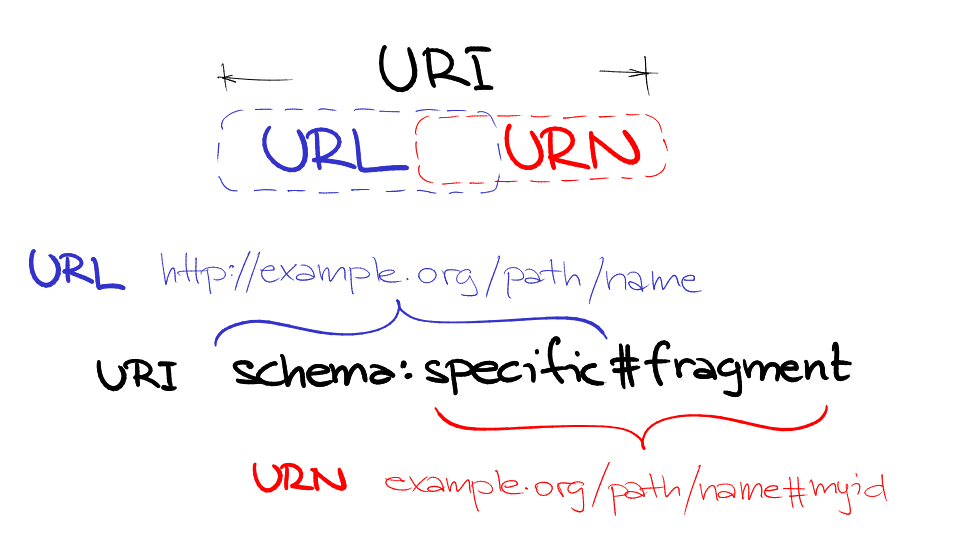
\includegraphics[width=0.8\textwidth]{img/screenshot_2025-04-25_11-53-53.png}
    \caption{URI, URL, URN}
\end{figure}

Všeobecně můžeme mluvit o 3 hlavních verzích HTTP protokolu:

\begin{table*}[h]
    \centering
    \begin{tabular}{|c|c|c|c|}
        \hline
        Vlastnost & HTTP/1.1 & HTTP/2 & HTTP/3 \\
        \hline
        Multiplexace & Ne & Ano (1 TCP spojení) & Ano (QUIC – UDP) \\
        \hline
        Binární protokol & Ne (textový) & Ano & Ano \\
        \hline
        Server push & Ne & Ano & Ano \\
        \hline
        Prioritizace & Ne & Ano & Ano \\
        \hline
        Transportní protokol & TCP & TCP & QUIC (UDP) \\
        \hline
    \end{tabular}
    \caption{Srovnání verzí HTTP}
\end{table*}

\subsubsection*{Komunikace klient-server}

\begin{figure}[H]
    \centering
    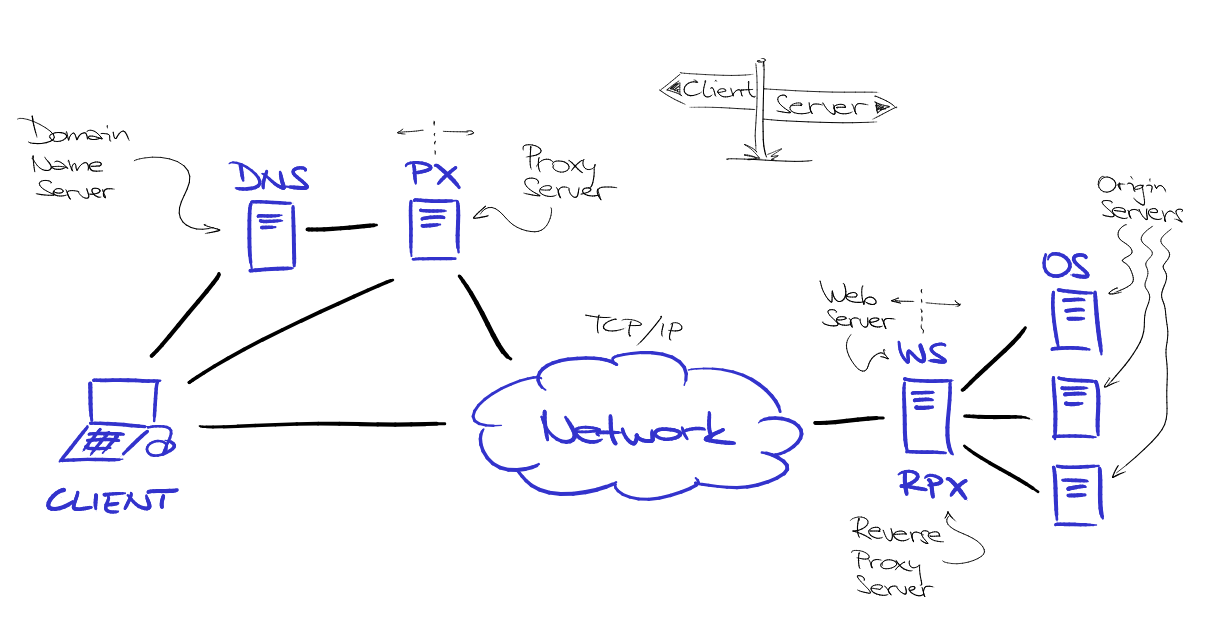
\includegraphics[width=1\textwidth]{img/screenshot_2025-04-25_21-05-04.png}
    \caption{Komunikace klient server přes internet}
\end{figure}

%% Námět na ANKI:
% Co je DNS, co je proxy, co je reverse proxy, co je origin server a jak to spolu dohromady funguje, jak vypadá struktura http požadavku a odpovědi

Ukázkový HTTP POST požadavek:

\lstdefinelanguage{HTTP}{
  morekeywords={GET,POST,PUT,DELETE,HTTP/1.1,Host,Content-Type,User-Agent},
  sensitive=true,
  morecomment=[l][\color{gray}]{//},
  morestring=[b]",
}

\begin{lstlisting}[language=HTTP]
POST /api/v1/users HTTP/1.1
Host: example.com
Content-Type: application/json
{
    "username": "example",
    "password" "password"
}
\end{lstlisting}

Ukázková odpověď serveru:
\begin{lstlisting}[language=HTTP]
HTTP/1.1 200 OK
{
    "status": "success",
    "data": {
        "userId": 123,
        "username": "example"
    }
}
\end{lstlisting}

\subsubsection*{HTTP hlavičky}
HTTP hlavičky jsou klíčové pro přenos metadat mezi klientem a serverem. Obsahují informace o požadavku nebo odpovědi, jako jsou typ obsahu, jazyk, délka obsahu atd.

Příklady běžně používaných hlaviček:
\begin{itemize}
    \item \textbf{User-Agent}: Informace o prohlížeči nebo aplikaci, která požadavek odesílá.
    \item \textbf{Content-Type}: Typ obsahu, který je odesílán (např. application/json).
    \item \textbf{Accept}: Typy obsahu, které klient akceptuje.
    \item \textbf{Authorization}: Ověření identity uživatele (např. pomocí tokenu).
    \item \textbf{Cookie}: Odesílání cookies mezi klientem a serverem.
    \item \textbf{Set-Cookie}: Odpověď serveru, která nastavuje cookie na straně klienta.
    \item \textbf{Cache-Control}: Řízení mezipaměti (např. no-cache, max-age).
    \item \textbf{Location}: Používá se při přesměrování (status kód 3xx) a obsahuje URL, na kterou má být klient přesměrován.
    \item \textbf{Content-Length}: Délka obsahu v bajtech.
    \item \textbf{Connection}: Řízení spojení (např. keep-alive, close).
    \item \textbf{Origin}: Původní doména, ze které byl požadavek odeslán (používá se při CORS).
    \item \textbf{Referer}: URL stránky, ze které byl požadavek odeslán.
    \item \textbf{Accept-Encoding}: Typy kódování, které klient akceptuje (např. gzip, deflate).
    \item \textbf{Accept-Language}: Jazykové preference klienta (např. en-US, cs-CZ).
\end{itemize}

\subsubsection*{HTTP status kódy}
Tyto kódy informují klienta o výsledku požadavku a mohou být rozděleny do několika kategorií:

\begin{itemize}
    \item \textbf{1xx (Informational)}: Informace o průběhu požadavku (např. 100 Continue).
    \item \textbf{2xx (Success)}: Úspěšné zpracování požadavku (např. 200 OK, 201 Created).
    \item \textbf{3xx (Redirection)}: Přesměrování na jinou URL (např. 301 Moved Permanently, 302 Found).
    \item \textbf{4xx (Client Error)}: Chyba na straně klienta (např. 400 Bad Request, 401 Unauthorized, 404 Not Found).
    \item \textbf{5xx (Server Error)}: Chyba na straně serveru (např. 500 Internal Server Error, 502 Bad Gateway).
\end{itemize}

\subsubsection*{HTTP metody}
HTTP protokol podporuje různé metody, které určují typ operace, kterou klient požaduje provést na serveru. 

\begin{itemize}
    \item \textbf{GET}: Získání dat ze serveru. Neposílá žádná data v těle požadavku.
    \item \textbf{HEAD}: Získání hlaviček odpovědi bez těla. Používá se k ověření existence zdroje.
    \item \textbf{POST}: Odeslání dat.
    \item \textbf{PUT}: Aktualizace existujícího zdroje nebo vytvoření nového. Je idempotentní, což znamená, že opakované volání stejného požadavku má stejný efekt jako jednorázové.
    \item \textbf{DELETE}: Odstranění zdroje.
    \item \textbf{OPTIONS}: Získání informací o dostupných metodách pro daný zdroj. Často se používá pro CORS (Cross-Origin Resource Sharing).
\end{itemize}

\subsubsection*{Bezpečnostní aspekty}

HTTP protokol sám o sobě nepoužívá šifrování, což znamená, že data přenášená mezi klientem a serverem mohou být snadno odposlouchávána třetími stranami. Pro zajištění bezpečnosti se používá HTTPS, což je HTTP protokol běžící nad šifrovaným kanálem TLS/SSL.

HTTPS zajišťuje:
\begin{itemize}
    \item Šifrování dat mezi klientem a serverem.
    \item Ověření identity serveru pomocí certifikátů.
    \item Integritu dat, což znamená, že data nemohou být změněna během přenosu.
\end{itemize}
